\documentclass[10pt, oneside]{article}
\usepackage[a4paper, total={5.5in, 9in}]{geometry}
\usepackage[ngerman]{babel}
\usepackage{import}

\import{../.texit/include}{preamble}

\title{Angewandte Logik\\[15pt]\Large{Hausaufgabenblatt 1}\\[10pt]\Large{SoSe 2025}}
\author{Volodymyr But\\[5pt][Matrikel-Nr.: 982324]\\[10pt]Hochschule Trier}
\date{}

% - - - - - - - - - - - - - - - - - - - - - - - - - - - - - - - - - - - - - - %

\begin{document}

\maketitle
\vspace{25px}

\section{Aufgabe 1}

Gegeben sei folgende Information:
\begin{enumerate}[1.]
    \item A oder C ist wahr.
    \item A gilt genau dann, wenn B gilt.
    \item Wenn B und C gelten, dann gilt auch D.
\end{enumerate}
Formulieren Sie diese Zusammenh"ange als Formeln der Aussagenlogik.
\begin{enumerate}[1.]
    \item $A \lor B$
    \item $A \Leftrightarrow B$
    \item $B \land C \Rightarrow D$
\end{enumerate}

\section{Aufgabe 2}

\begin{enumerate}[(a)]
    \item Beschreiben Sie folgende Formel mit einer Baumstruktur:

        $(\lnot A \Rightarrow (B \Leftrightarrow C)) \land ((A \land C) \Rightarrow \lnot D)$

        Siehe Abbildung~\ref{fig:ha.01.2.a.1}

    \item Propagieren Sie die Wahrheitswerte im Baum f"ur die Interpretation

        \verb|A = f, B = w, C = f, D = w|

        Siehe Abbildung~\ref{fig:ha.01.2.a.2}
\end{enumerate}

\pagebreak
\section{Aufgabe 3}

Überprüfen Sie folgende Formeln hinsichtlich Allgemeingültigkeit,
Erfüllbarkeit, Falsifizierbarkeit und Unerfüllbarkeit

\begin{enumerate}[(a)]
    \item $X := \lnot((A \lor B) \land (\lnot B \lor C)))$

        \begin{table}[h]
            \hspace{23px}
            \begin{tabular}{|c|c|c|c|}
                \hline
                A & B & C & $X$ \\
                \hline
                w & w & w & f \\
                \hline
                w & w & f & w \\
                \hline
                w & f & w & f \\
                \hline
                w & f & f & f \\
                \hline
                f & w & w & f \\
                \hline
                f & w & f & w \\
                \hline
                f & f & w & w \\
                \hline
                f & f & f & w \\
                \hline
            \end{tabular}
        \end{table}

        \verb|Allgemeingültigkeit: nein| \\
        \verb|Erfüllbarkeit:       ja| \\
        \verb|Falsifizierbarkeit:  ja| \\
        \verb|Unerfüllbarkeit:     nein|

    \item $X := ((A \Rightarrow (B \Rightarrow C)) \Rightarrow ((A \Rightarrow B) \Rightarrow (A \Rightarrow C)))$

        \begin{table}[h]
            \hspace{22px}
            \begin{tabular}{|c|c|c|c|}
                \hline
                A & B & C & $X$ \\
                \hline
                w & w & w & w \\
                \hline
                w & w & f & w \\
                \hline
                w & f & w & w \\
                \hline
                w & f & f & w \\
                \hline
                f & w & w & w \\
                \hline
                f & w & f & w \\
                \hline
                f & f & w & w \\
                \hline
                f & f & f & w \\
                \hline
            \end{tabular}
        \end{table}

        \verb|Allgemeingültigkeit: ja| \\
        \verb|Erfüllbarkeit:       ja| \\
        \verb|Falsifizierbarkeit:  nein| \\
        \verb|Unerfüllbarkeit:     nein|
\end{enumerate}

\begin{figure}[p]
    \centering
    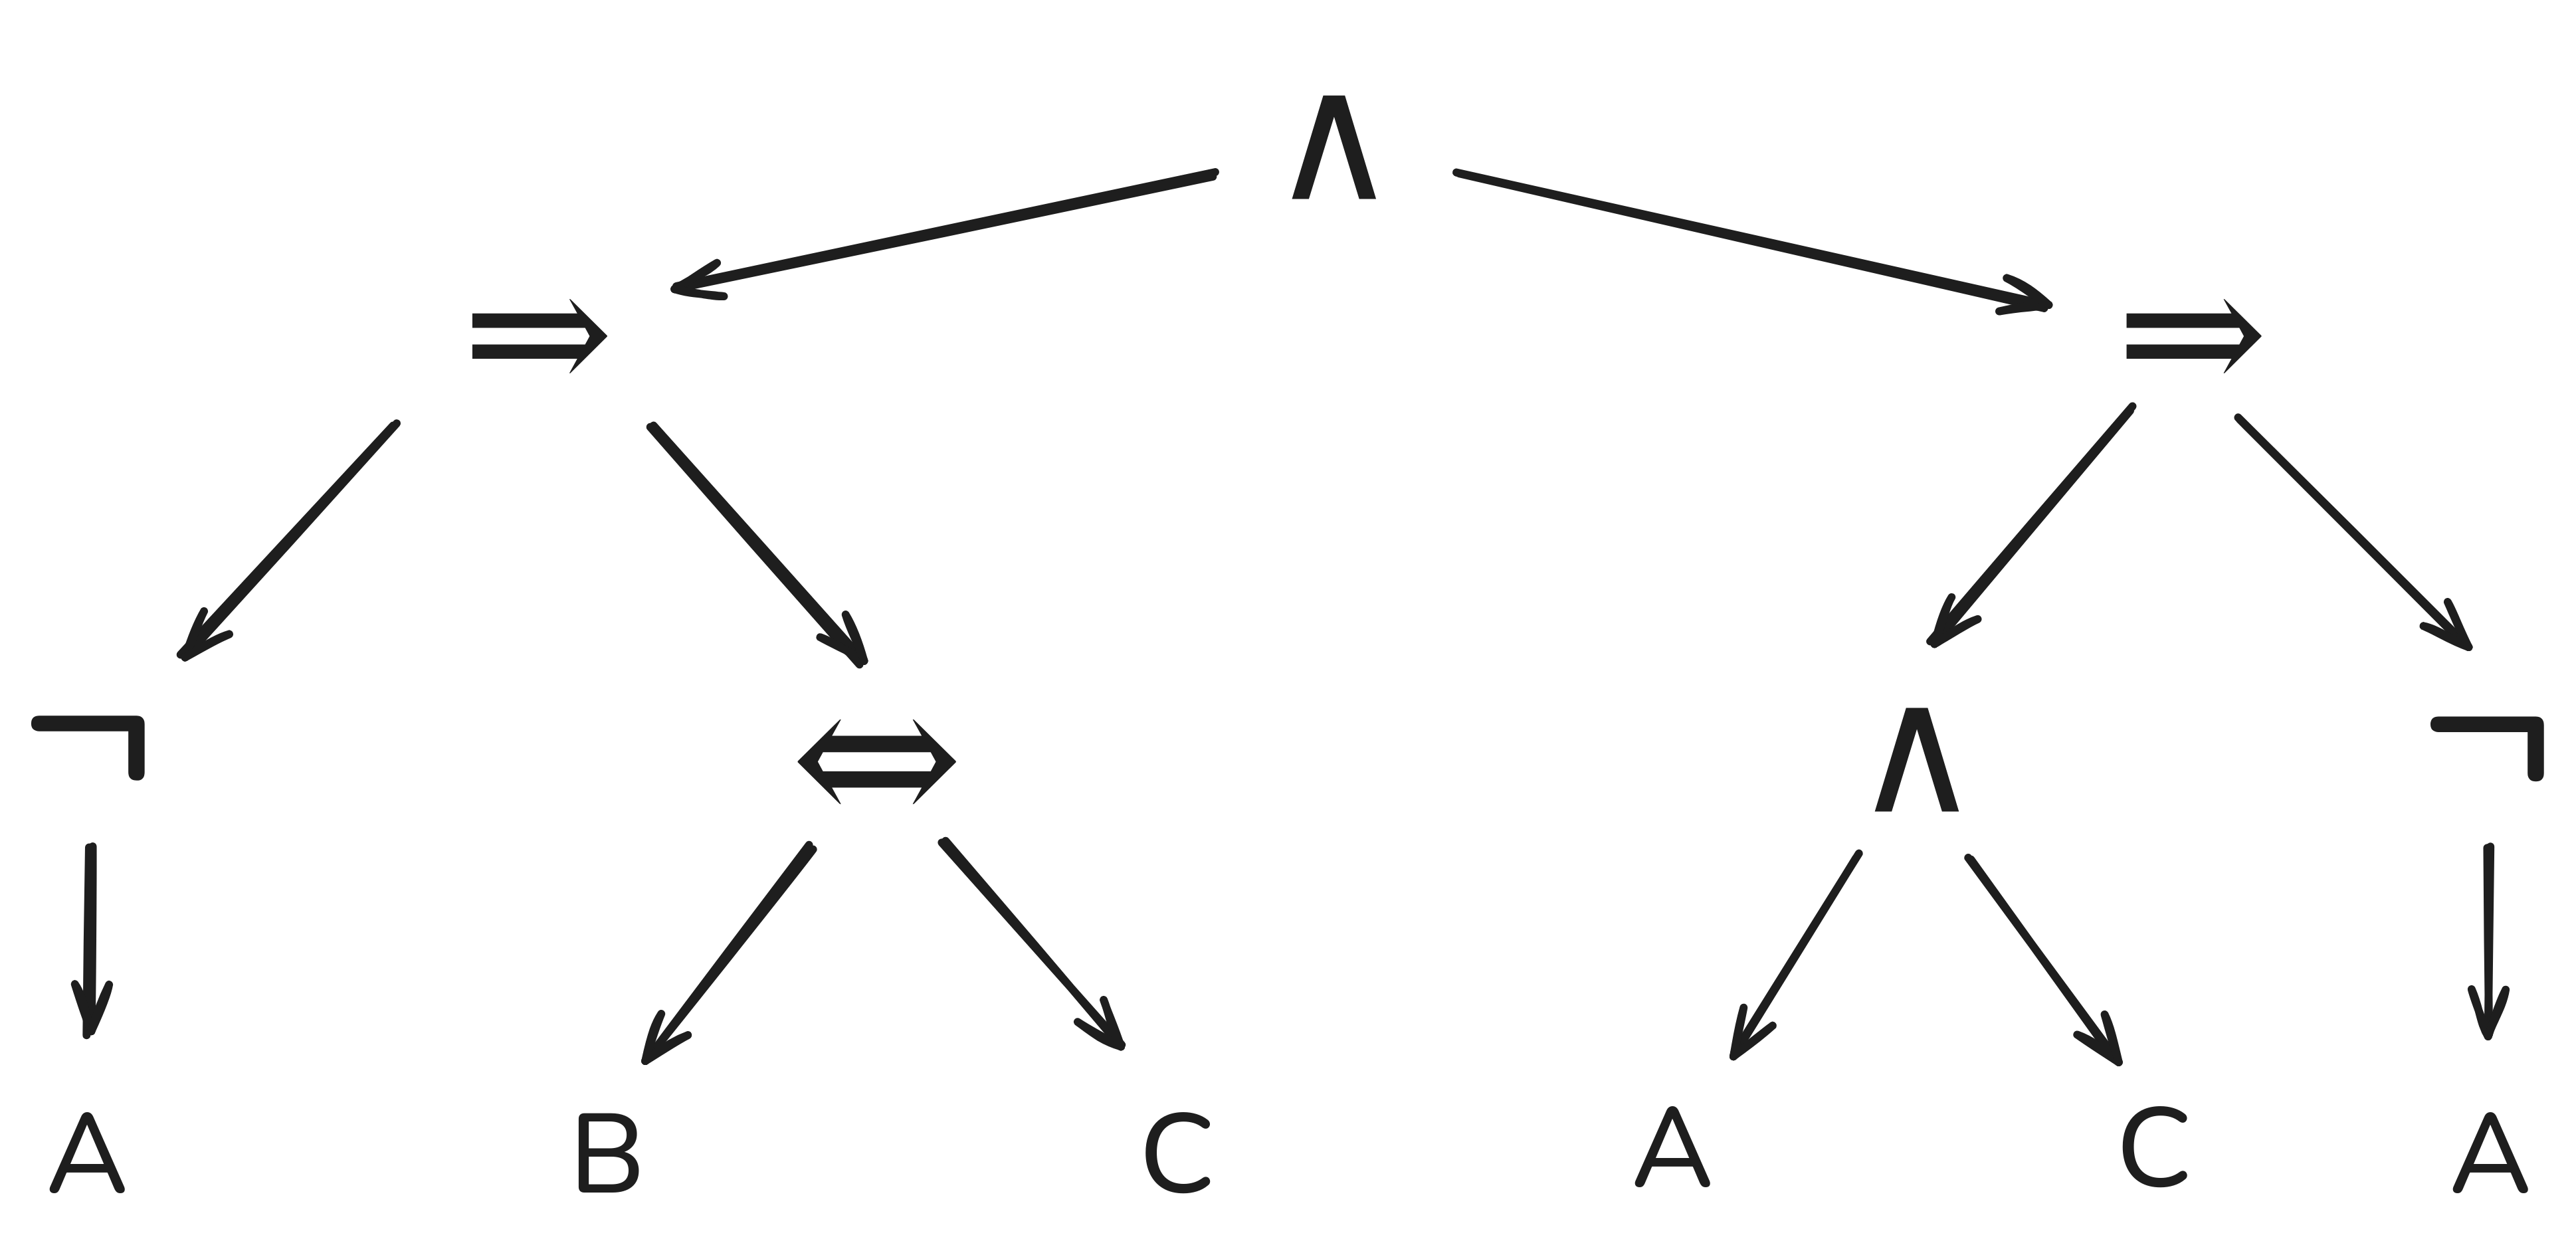
\includegraphics[width=1\textwidth]{./assets/ha.01.2.a.1.png}
    \caption{}
    \label{fig:ha.01.2.a.1}
\end{figure}

\begin{figure}[p]
    \centering
    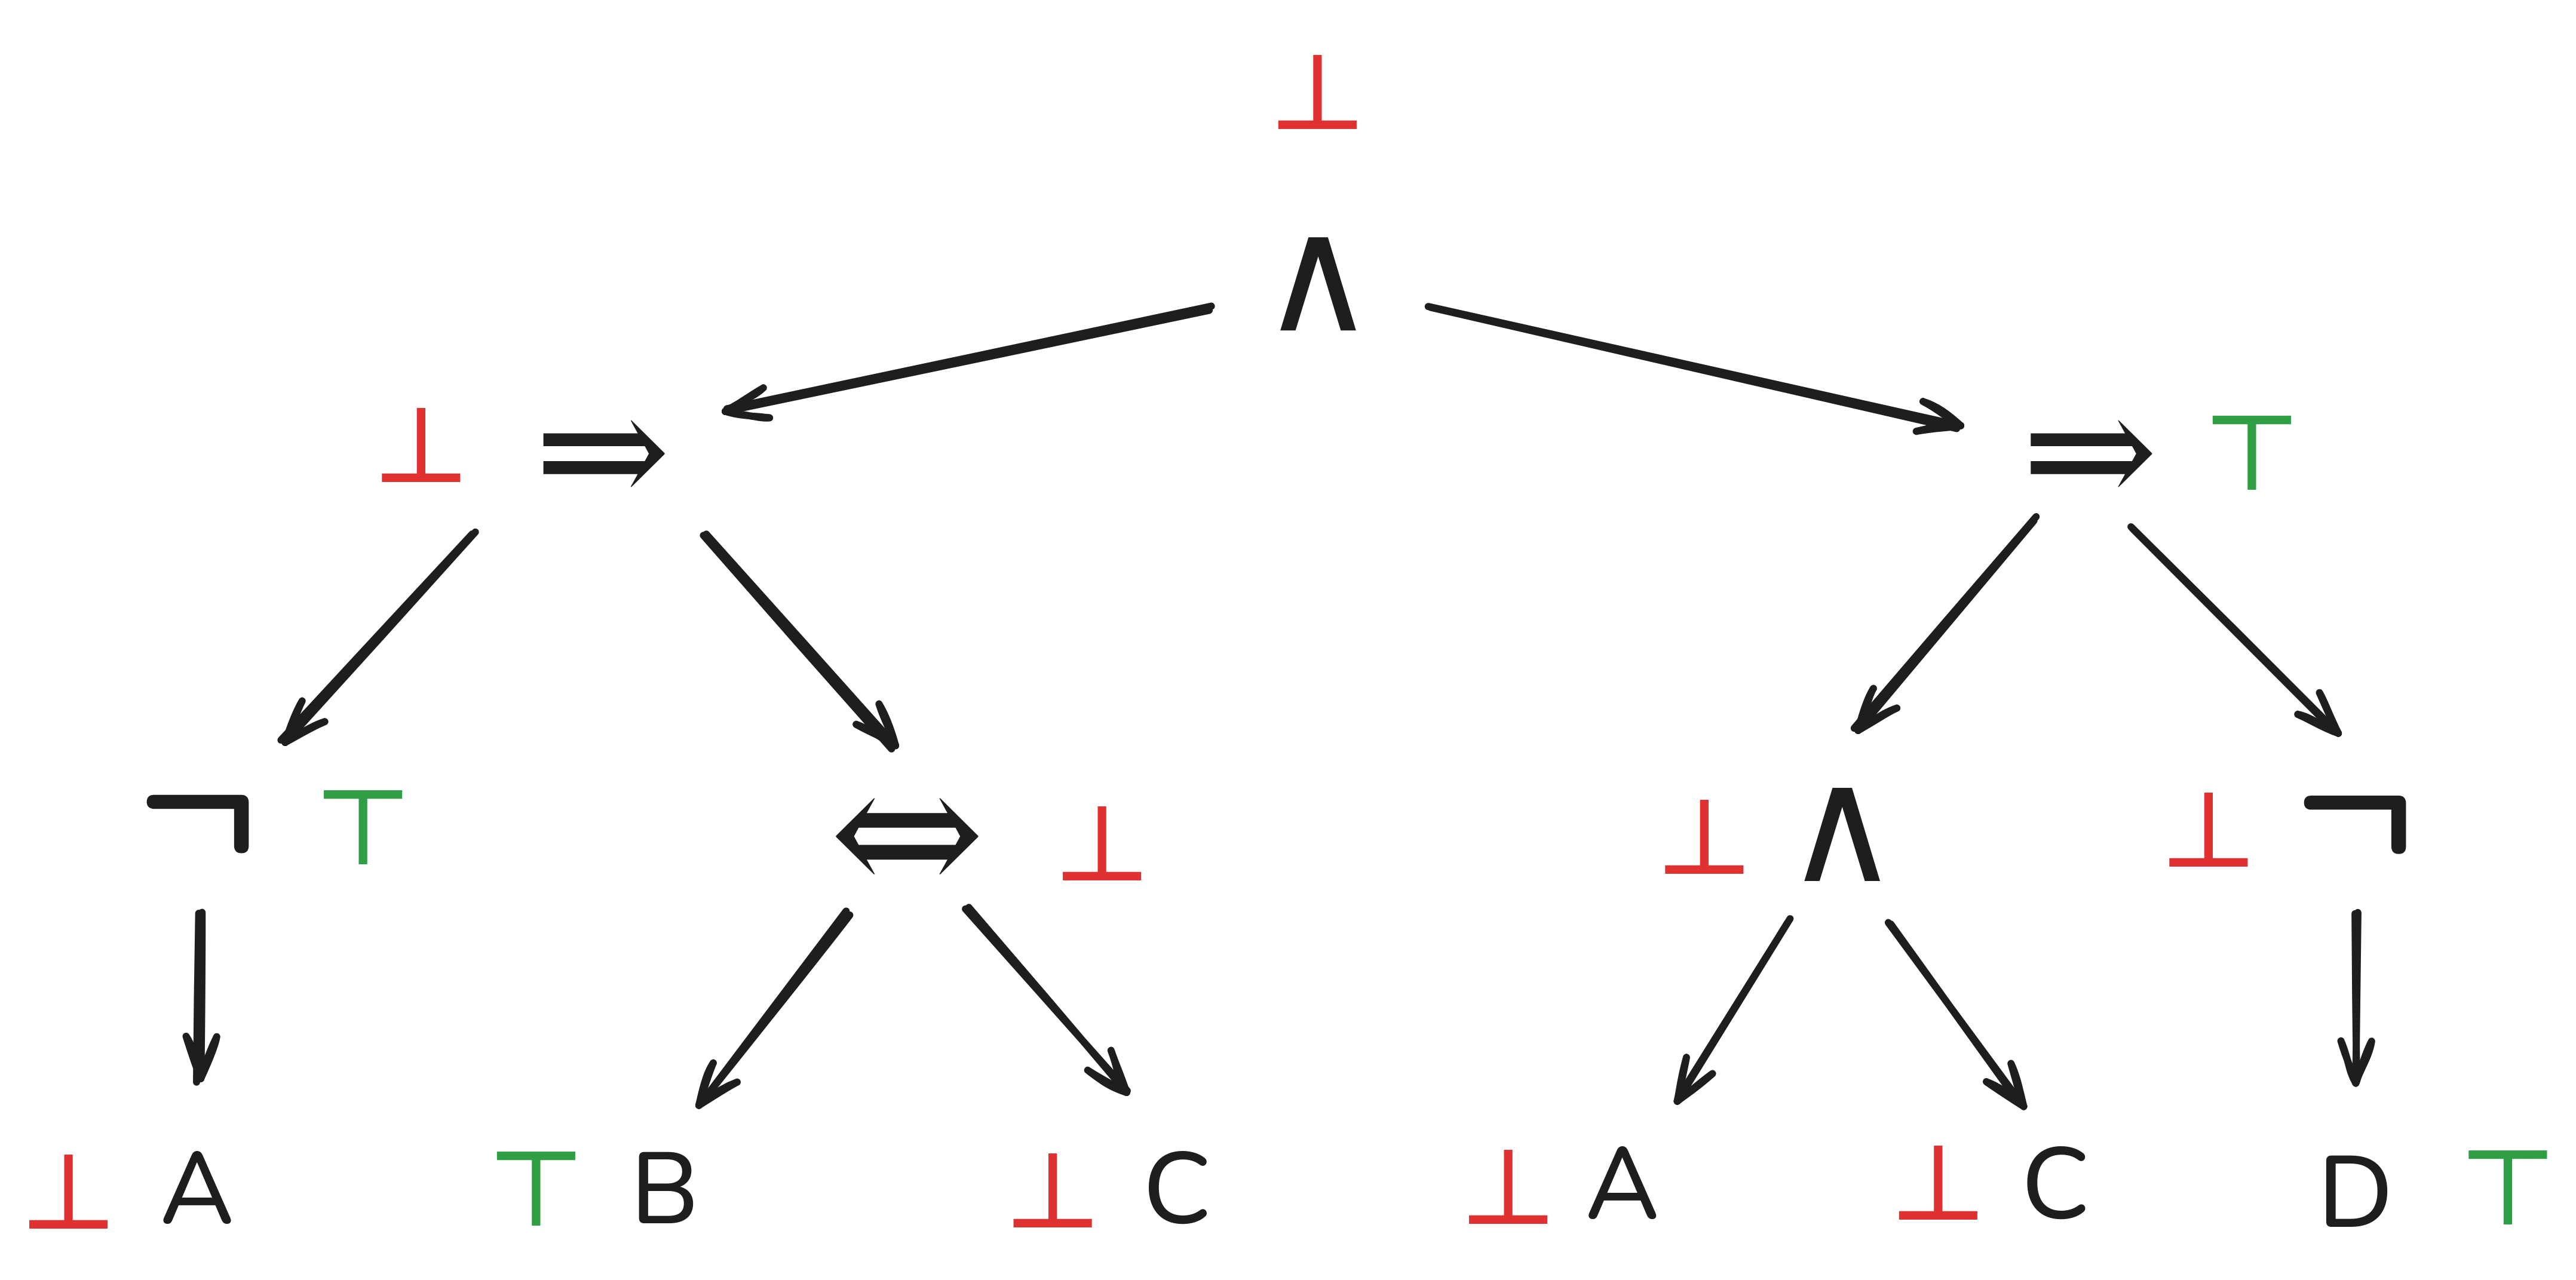
\includegraphics[width=1\textwidth]{./assets/ha.01.2.a.2.png}
    \caption{}
    \label{fig:ha.01.2.a.2}
\end{figure}

\end{document}
